\begin{figure}[t]
\centering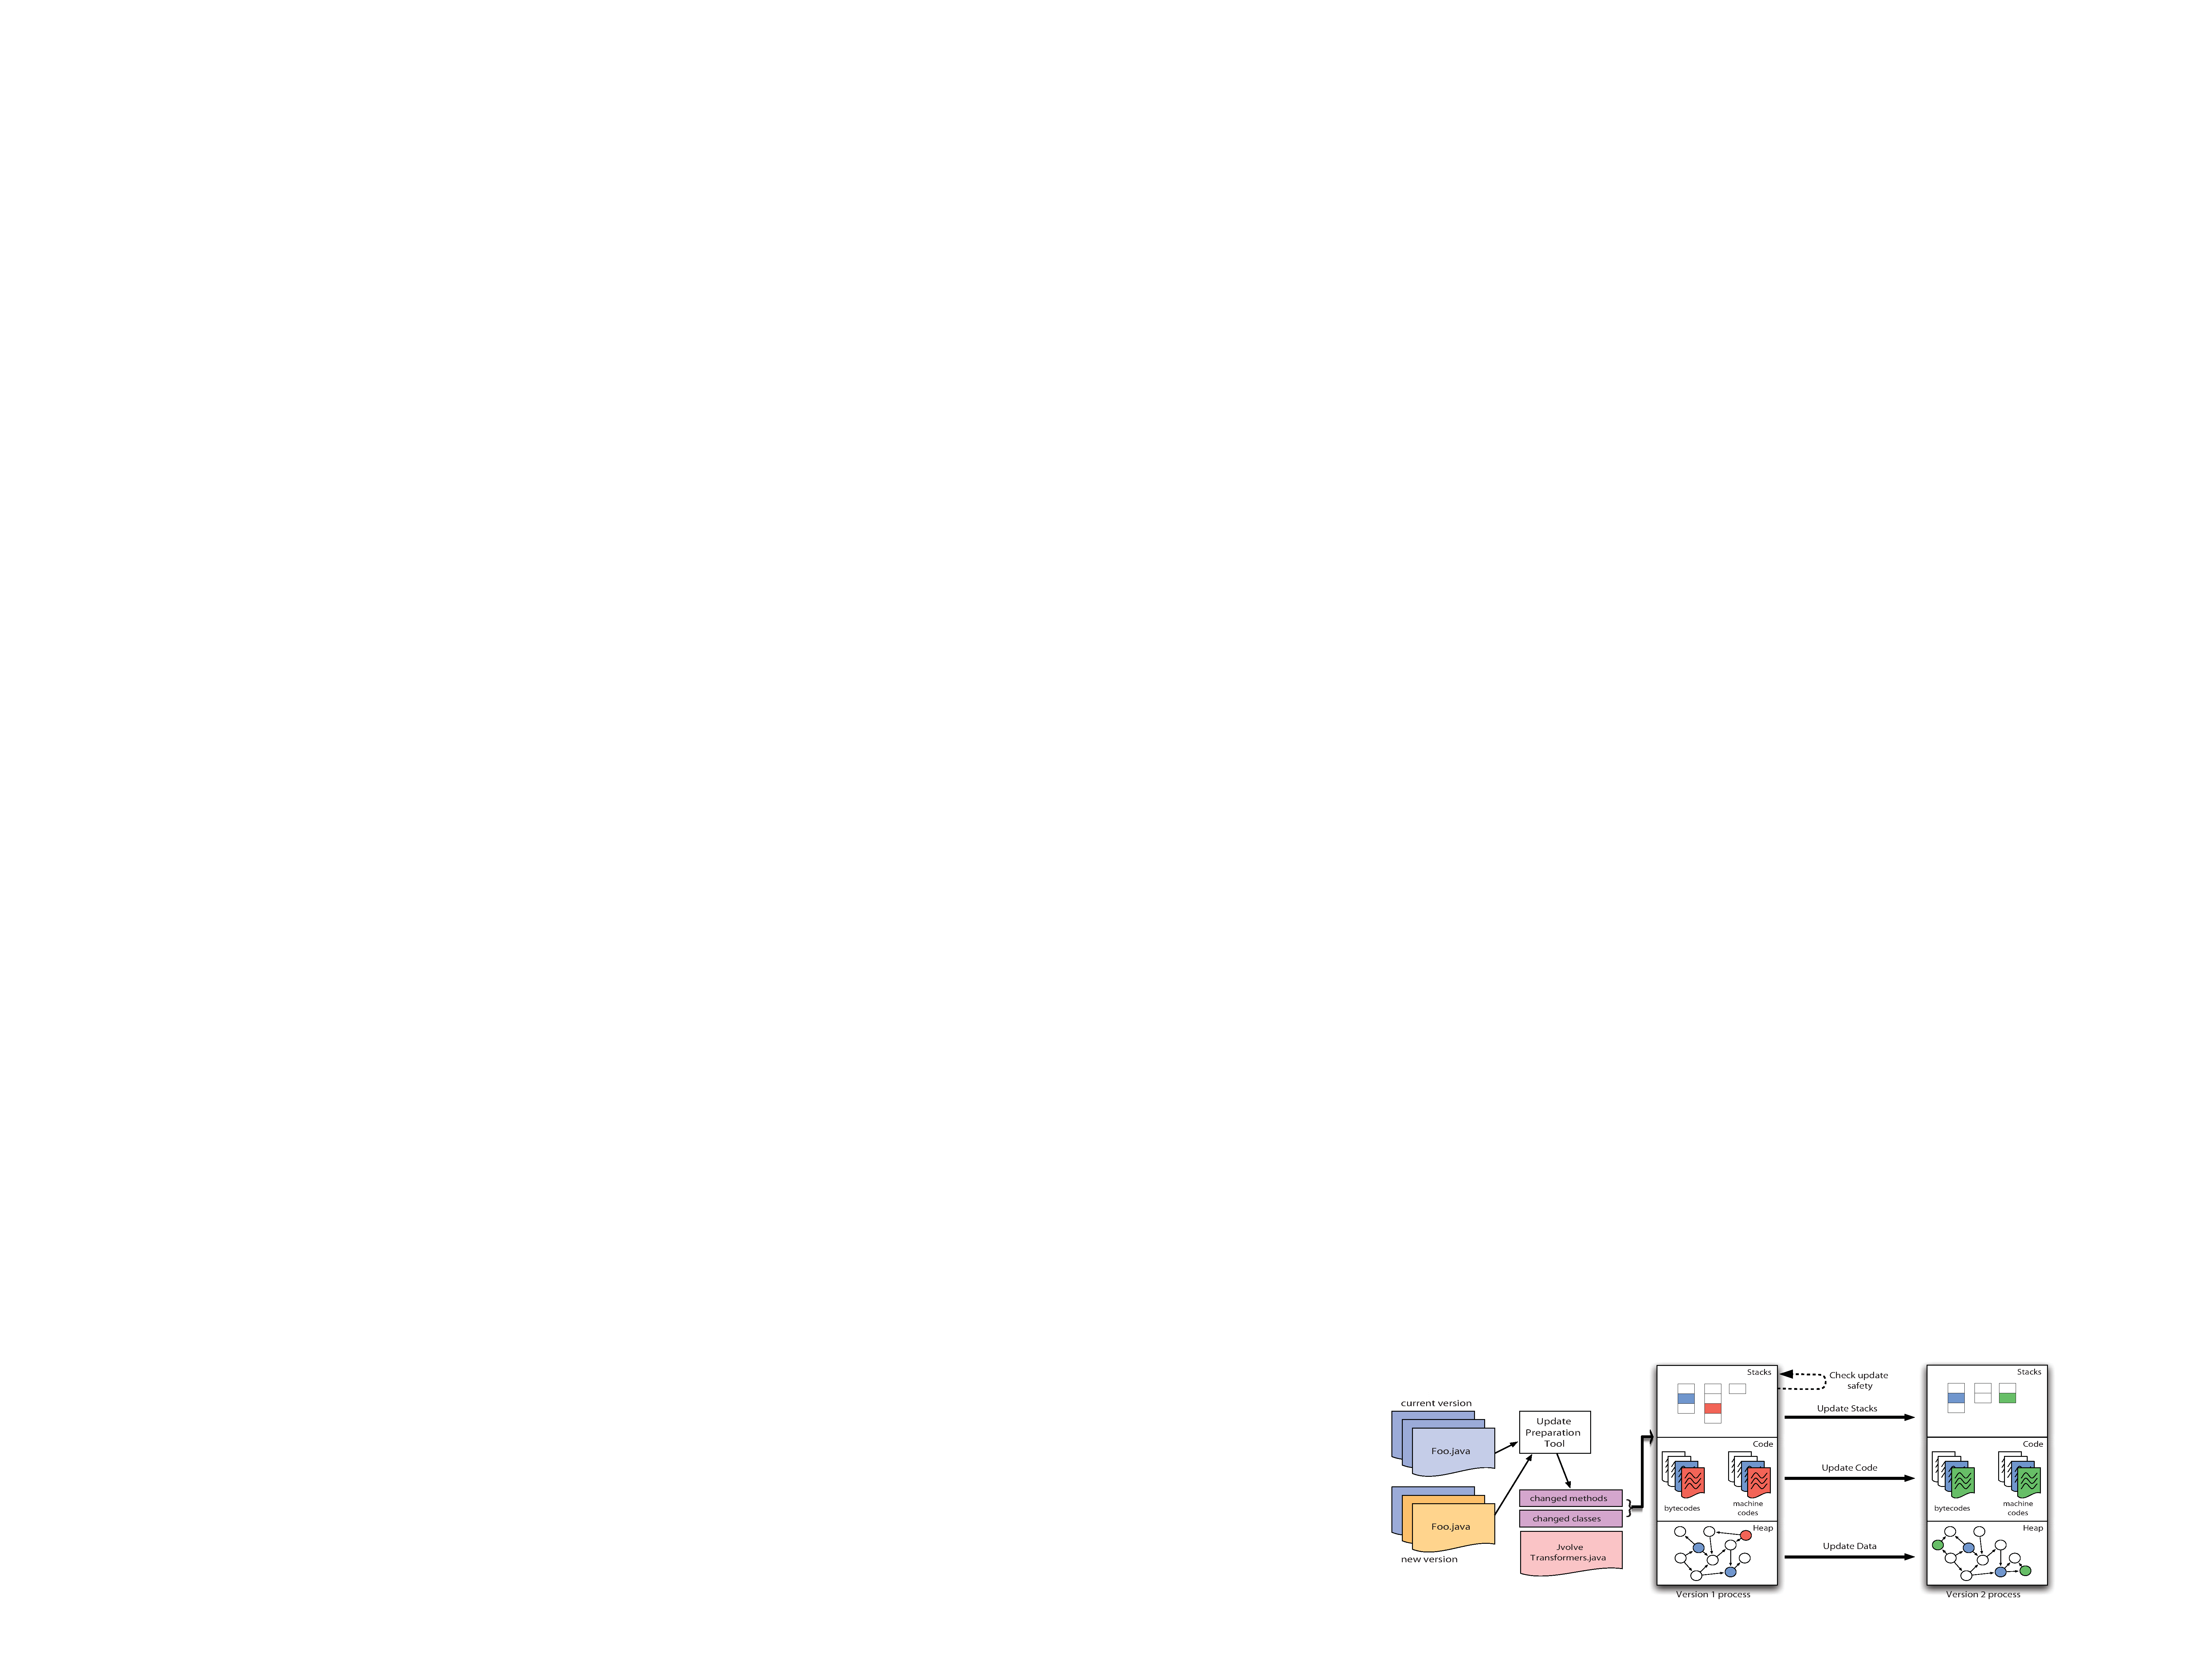
\includegraphics[scale=0.38,clip=true,trim=2170 90 250 2125]{100-images/PASS-HPC-poster-8-2009-cropped}
\caption{Overview of the Dynamic Updating process.\label{fig:overview}}
\end{figure}

\section{Introduction}
\label{sec:system-intro}

Figure~\ref{fig:overview} illustrates the dynamic updating process. The left
portion depicts the work done offline. The developer writes the old and new
versions of the application, and tests them as part of the software
development process. The \acf{UPT} examines source code
of the old and new versions of the application and prepares a dynamic patch.
The user feeds the patch to a process with dynamic-updating support,
depicted on the right. The figure shows two processes, one
running version one of an application, showing stacks, code and heap; and
another running version two of the same application. The goal is to
transition from a process running an old version of the application, to one
running the new version, on the fly, without stopping and restarting the
application.

We assume that developers write and fully test both the old and new
versions using standard development practices without anticipating that
the application is going to be updated dynamically. Testing is already a
well established part of software development. With dynamic updating,
developers should test the update process, in addition to testing their
applications.
When it comes time to
perform the update, the developer provides the source code for the old and
new versions to \JV's \acf{UPT}. The \acs{UPT} compares these two versions
and provides a specification for the update. The specification consists of
two major parts. First, it contains information about code changes that
inform the VM when it is safe to perform the update, what old
methods to invalidate, and what new method bodies to load. Second, it
informs the VM how to deal with changes to data. The VM uses this
specification to transform classes and objects in the heap to conform to
their new version. The programmer has the option to
modify the update specification. Specifically, the
\acs{UPT} does not reason deeply about the semantics of
data structure changes. The programmer may need to modify the \acs{UPT}s
output to obtain a correct program.

Given an update specification, the user
signals the running VM to apply the update.  The VM loads the new class
files and schedules the update. The VM scheduler signals an interrupt, which
stops all threads at VM safe points, where it is safe to perform thread
scheduling and garbage collection. \JV then checks if the VM is at a
\emph{DSU safe point}. DSU safe points require that no thread's activation
stack contains a \emph{restricted} method, which is part of the specification.

Restricted methods are of three categories: (1) methods changed by the
update, (2) methods whose bytecode is unchanged but whose compiled
representation may change, and (3) methods specified by the user or
testing process for semantic reasons. If
restricted methods are on stack, the VM installs return-barriers for~(1)
and~(3), and performs on-stack-replacement for~(2) to reach a DSU safe
point.  Section~\ref{sec:safe} describes how \JV reaches a safe point in
detail.

Once all application threads have synchronized at DSU safe points, \JV
applies the update. It first invalidates the compiled versions of all
changed methods.  These methods are recompiled as needed---the adaptive JIT
compiler will generate code the next time the program invokes an
invalidated method, and will optimize it further, if the program executes it
frequently enough.  The VM then initiates a full copying garbage collection. It
piggybacks on the garbage collector to detect all existing objects whose
classes change. It allocates objects that conform to the new class
definitions.
Finally, after garbage collection, \JV performs class and
object transformations to populate per-class static fields and per-object
instance fields with valid state.  At this point, the update is complete.

\section{Performance}
\label{sec:performance}

\JV's impact on performance can be divided into the following. 1) the
steady state impact of implementing dynamic updating support, 2) the pause
in application execution to perform the update, and 3) the cost of
recompiling updated and invalidated methods upon resuming execution. The
latter is very hard to measure and can be grouped with the steady state
performance impact. Our experiments show that
the main performance impact of \JV is the pause time while applying an update. Once
updated, the application eventually runs without further overhead.  To
confirm this claim, we measured the throughput and latency of two 
Jetty versions while running on
stock \RVM and on \JV after dynamically updating to the next version.
Section~\ref{subsec:jetty-webserver-performance} shows that the performance of these
configurations is essentially identical.

% We report
% on this experiment in Section~\ref{subsec:jetty-perf}.

The cost of applying an update is the time to load any new classes, invoke
a full heap garbage collection, and apply the transformation methods on
objects belonging to updated classes.  Roughly, the time to suspend threads
and check that the application is at a safe-point is less than a
millisecond, and classloading time is usually less than 20ms.
The update disruption time is primarily due to the GC and
object transformers, and is proportional to the size of the heap and the
fraction of objects being transformed.  We wrote a simple microbenchmark to
measure these overheads.  The results reported in
Section~\ref{subsec:microbench} show that object transformation
is the dominant cost.

We conducted all our experiments on an Intel Core 2 Quad machine running at
2.4 GHz machine with 2 GB of RAM.  The machine ran Ubuntu 7.10 on Linux
kernel version 2.6.22. We implemented \JV on top of \RVMversion and built a
FullAdaptiveSemiSpace configuration of the \VM. The FullAdaptive
configuration means that the \VM's code is compiled at the highest level of
optimization while creating the \VM's boot image (Full) and the application
code is compiled adaptively adaptively (Adaptive)~\cite{AAB+:00}. In
adaptive compilation, the \VM baseline compiles an application method the
first time it is executed, and recompiles the method at increasing levels
of optimization as it gets invoked more often.  The SemiSpace configuration
refers to \RVM's semi-space garbage collector.

% \begin{figure}[t]
\begin{small}
\begin{center}
\begin{tabular}{|l|c|c|c|c|} \hline \T
Config.                & \multicolumn{2}{c|}{Throughput (MB/s)}  & \multicolumn{2}{c|}{Latency (ms)} \\ \cline{2-5}
                       & Median   & Quartiles \T                 & Median & Quartiles                \\ \hline \T
\JikesRVM{}            & 122.437  & 121.44--123.32               & 0.442  & 0.394--0.496             \\
\DSU{}                 & 121.308  & 121.12--121.41               & 0.349  & 0.341--0.351             \\
\DSU{} upd             & 121.242  & 121.09--121.29               & 0.345  & 0.341--0.349             \\ \hline
\end{tabular}
\end{center}
\end{small}
% \caption{Throughput and latency measurements for Jetty webserver v5.1.6
% showing median and semi-interquartile range\label{tab:jetty}}
\begin{center}
\scalebox{0.63}{\includegraphics{graphs/jetty-throughput-latency}}
\caption{Throughput and latency measurements of Jetty webserver v5.1.6\label{fig:jetty}}
\end{center}
\end{figure}

% \begin{figure}[t]
\begin{center}
\scalebox{0.63}{\includegraphics{graphs/jetty-throughput-latency}}
\caption{Throughput and latency measurements of Jetty webserver v5.1.6\label{fig:jetty}}
\end{center}
\end{figure}

% \begin{table*}[t]
\begin{footnotesize}
\begin{center}
\begin{tabular}{|r|r|rrrrrrrrrrr|}
                                                                                                                                   \hline
\multirow{2}{*}{\# objects}     & \multicolumn{1}{c}{Heap}   & \multicolumn{11}{|c|}{Fraction of updated objects \T}            \\
                                & \multicolumn{1}{c|}{size}  &
                       0\%  &   10\%  &   20\%  &   30\%  &   40\%  &   50\%  &   60\%  &   70\%  &   80\%  &   90\%  &  100\%  \\ \hline
\multicolumn{13}{|c|}{Garbage collection time (ms) \T}                                                                          \\ \hline \T
 280000 &  160 MB &    78.2 &    81.3 &    83.1 &    89.3 &    99.0 &   103.2 &   108.3 &   113.2 &   113.3 &   120.3 &   120.0 \\
 770000 &  320 MB &   148.9 &   165.0 &   181.9 &   195.8 &   213.2 &   223.2 &   237.0 &   249.0 &   262.0 &   269.5 &   278.6 \\
1760000 &  640 MB &   313.3 &   347.7 &   382.9 &   416.0 &   449.8 &   478.9 &   506.8 &   534.0 &   558.8 &   583.7 &   601.5 \\
3670000 & 1280 MB &   615.4 &   694.6 &   763.0 &   833.6 &   900.1 &   965.9 &  1019.0 &  1076.4 &  1129.9 &  1181.2 &  1217.5 \\ \hline
\multicolumn{13}{|c|}{Running transformation functions (ms) \T}                                                                 \\ \hline \T
 280000 &  160 MB &     0.1 &    13.0 &    23.2 &    34.6 &    43.9 &    54.0 &    62.7 &    74.5 &    84.1 &    93.9 &   104.2 \\
 770000 &  320 MB &     0.1 &    33.7 &    63.1 &    91.2 &   116.8 &   145.4 &   173.9 &   201.0 &   231.3 &   262.0 &   292.6 \\
1760000 &  640 MB &     0.1 &    77.9 &   143.9 &   207.7 &   269.5 &   333.7 &   397.6 &   464.0 &   534.6 &   604.5 &   674.9 \\
3670000 & 1280 MB &     0.1 &   160.8 &   299.2 &   429.4 &   560.2 &   693.8 &   827.3 &   975.0 &  1119.6 &  1263.7 &  1405.4 \\ \hline
\multicolumn{13}{|c|}{Total DSU pause time (ms) \T}                                                                             \\ \hline \T
 280000 &  160 MB &    82.8 &    99.0 &   109.5 &   128.0 &   147.6 &   161.2 &   174.5 &   192.8 &   202.5 &   218.8 &   228.1 \\
 770000 &  320 MB &   153.6 &   202.9 &   249.0 &   291.4 &   334.5 &   372.6 &   414.8 &   455.4 &   498.1 &   535.3 &   576.8 \\
1760000 &  640 MB &   316.6 &   429.5 &   530.5 &   627.2 &   723.4 &   816.0 &   908.6 &  1002.6 &  1097.5 &  1191.5 &  1281.2 \\
3670000 & 1280 MB &   618.7 &   859.0 &  1065.9 &  1269.9 &  1466.1 &  1663.6 &  1850.8 &  2054.2 &  2253.1 &  2448.5 &  2627.9 \\ \hline
\end{tabular}
\end{center}
\end{footnotesize}
\caption{Microbenchmark results: \DSU{} update pause time (in ms) for various heap sizes}
\label{tab:microbench}
\end{table*}


\begin{figure}[t]
\centering
\begin{small}
\begin{tabular}{lcccc} \toprule
\multirow{2}{*}{Config.} & \mc{2}{c}{Throughput (MB/s)}  & \mc{2}{c}{Latency (ms)} \\ \cmidrule{2-5}
           & Median   & Quartiles                    & Median & Quartiles     \\ \midrule
%            & \mc{2}{c}{Throughput (MB/s)}  & \mc{2}{c}{Latency (ms)} \\ \cmidrule{2-5}
% Config.    & Median   & Quartiles                    & Median & Quartiles     \\ \midrule
\RVM       & 122.437  & 121.44--123.32               & 0.442  & 0.394--0.496  \\
\JV        & 121.308  & 121.12--121.41               & 0.349  & 0.341--0.351  \\
\JV upd.   & 121.242  & 121.09--121.29               & 0.345  & 0.341--0.349  \\ \bottomrule
\end{tabular}
\end{small}
\\[2ex]
\includegraphics[scale=0.63]{100-graphs/jetty-throughput-latency}
% \caption{Throughput and latency measurements of Jetty webserver v5.1.6\label{fig:jetty}}
\hangcaption{Throughput and latency measurements for Jetty webserver
version 5.1.6 showing median and semi-interquartile range\label{fig:jetty}}
\VspaceFixForHangcaption
\end{figure}

% vim:tw=0


\subsection{Jetty Webserver performance}
\label{subsec:jetty-webserver-performance}

To see the effect of updating on application performance, we measured Jetty
under various request rates using httperf\index{httperf}, a webserver
benchmarking tool~\cite{httperf}, and determined Jetty's saturation rate to
be roughly 800 new connection requests/second. We then measured Jetty's
performance by issuing connections at this rate.  Each connection makes 5
serial requests for a 40 Kbyte file. Httperf reports average throughput and
average per-request latency over a 60 second period. We ran this experiment
21 times and report the median and quartiles of the throughput and latency
reports. With 21 runs, the range between the quartiles serves as a 98\%
confidence interval~\cite{PrattGibbons81}. In order to eliminate network
traffic effects, we ran the server on two cores of a quad-core machine and
the client on another core.

Figure~\ref{fig:jetty} shows our results in tabular form and plotted
graphically.  The second and third columns of the table report the median
throughput and the range between the two quartiles.  The third column and
fourth column report the median latency and the inter-quartile range.  The
first and second rows illustrate the performance of Jetty version 5.1.6
running on stock \RVM and \JV, respectively. The third row shows the
performance on \JV of Jetty 5.1.6 dynamically updated from version 5.1.5
prior to the start of the experiment.  The performance of the two \JV
configurations are statistically indistinguishable.  The two configurations'
corresponding inter-quartile ranges largely overlap.  The performance of
\JV is also quite similar to the performance of stock \RVM.  There are many
small differences between \JV and the stock implementation that change VM
code size, code layout, and garbage collection behavior. These differences
may impact performance directly and they may indirectly affect other
elements of the VM, such as the timing of garbage collections and JIT
optimizations (such indirect effects make VMs notoriously difficult to
benchmark~\cite{dacapo-cacm, diwan-measurement}).


\subsection{Microbenchmark performance}
\label{subsec:microbench}

The two dominant factors that determine \JV update time are the time to
perform a GC, determined by the number of objects, and the time to run
object transformers, determined by the fraction of objects being updated.
To measure each cost, we devised a simple microbenchmark that
creates an array of objects and transforms a specified fraction of these
objects when a dynamic software update is triggered. The microbenchmark has
two simple classes, \texttt{Change} and \texttt{NoChange}. Both contain
three integer fields, and three reference fields that are always {\tt
null}. The update adds an integer field to {\tt Change}. The user-provided
object transformation function copies the existing fields and initializes
the new field to zero.
% The benchmark contains two arrays, one for \texttt{Change} objects and
% one for \texttt{NoChange} objects.
We measure the cost of performing an update while varying the total number
of objects and the fraction of objects of each type. The number of objects
is the maximum that can fit in heap sizes 32, 64, 128 and 256 MB\@.  Note
that \RVM's heap includes \VM data structures as well. We measure the
running time in a generous heap, five times the minimum required size, such
that the only collections are those DSU triggers. We report the median of
21 runs.

% \begin{sidewaystable}
% \centering
% \begin{footnotesize}
% \begin{tabular}{|r|r|rrrrrrrrrrr|}
%                                                                                                                                    \hline
% \multirow{2}{*}{\# objects}     & \mc{1}{c}{Heap}   & \mc{11}{|c|}{Fraction of updated objects \T}                              \\
%                                 & \mc{1}{c|}{size}  &
%                        0\%  &   10\%  &   20\%  &   30\%  &   40\%  &   50\%  &   60\%  &   70\%  &   80\%  &   90\%  &  100\%  \\ \hline
% \mc{13}{|c|}{Garbage collection time (ms) \T}                                                                                   \\ \hline \T
%  280000 &  160 MB &    78.2 &    81.3 &    83.1 &    89.3 &    99.0 &   103.2 &   108.3 &   113.2 &   113.3 &   120.3 &   120.0 \\
%  770000 &  320 MB &   148.9 &   165.0 &   181.9 &   195.8 &   213.2 &   223.2 &   237.0 &   249.0 &   262.0 &   269.5 &   278.6 \\
% 1760000 &  640 MB &   313.3 &   347.7 &   382.9 &   416.0 &   449.8 &   478.9 &   506.8 &   534.0 &   558.8 &   583.7 &   601.5 \\
% 3670000 & 1280 MB &   615.4 &   694.6 &   763.0 &   833.6 &   900.1 &   965.9 &  1019.0 &  1076.4 &  1129.9 &  1181.2 &  1217.5 \\ \hline
% \mc{13}{|c|}{Running transformation functions (ms) \T}                                                                          \\ \hline \T
%  280000 &  160 MB &     0.1 &    13.0 &    23.2 &    34.6 &    43.9 &    54.0 &    62.7 &    74.5 &    84.1 &    93.9 &   104.2 \\
%  770000 &  320 MB &     0.1 &    33.7 &    63.1 &    91.2 &   116.8 &   145.4 &   173.9 &   201.0 &   231.3 &   262.0 &   292.6 \\
% 1760000 &  640 MB &     0.1 &    77.9 &   143.9 &   207.7 &   269.5 &   333.7 &   397.6 &   464.0 &   534.6 &   604.5 &   674.9 \\
% 3670000 & 1280 MB &     0.1 &   160.8 &   299.2 &   429.4 &   560.2 &   693.8 &   827.3 &   975.0 &  1119.6 &  1263.7 &  1405.4 \\ \hline
% \mc{13}{|c|}{Total DSU pause time (ms) \T}                                                                                      \\ \hline \T
%  280000 &  160 MB &    82.8 &    99.0 &   109.5 &   128.0 &   147.6 &   161.2 &   174.5 &   192.8 &   202.5 &   218.8 &   228.1 \\
%  770000 &  320 MB &   153.6 &   202.9 &   249.0 &   291.4 &   334.5 &   372.6 &   414.8 &   455.4 &   498.1 &   535.3 &   576.8 \\
% 1760000 &  640 MB &   316.6 &   429.5 &   530.5 &   627.2 &   723.4 &   816.0 &   908.6 &  1002.6 &  1097.5 &  1191.5 &  1281.2 \\
% 3670000 & 1280 MB &   618.7 &   859.0 &  1065.9 &  1269.9 &  1466.1 &  1663.6 &  1850.8 &  2054.2 &  2253.1 &  2448.5 &  2627.9 \\ \hline
% \end{tabular}
% \end{footnotesize}
% \caption{Microbenchmark results: \JV update pause time (in ms) for various heap sizes}
% \label{tab:microbench}
% \end{sidewaystable}

\begin{sidewaystable}
\newcommand{\GcTime}{\multirow{4}{0.15\textwidth}{Garbage collection time (ms)}}
\newcommand{\TfTime}{\multirow{4}{0.15\textwidth}{Running transformation functions (ms)}}
\newcommand{\ToTime}{\multirow{4}{0.15\textwidth}{Total DSU pause time (ms)}}
\centering \footnotesize
\begin{tabular}{*{14}{r}} \toprule
\mc{1}{c}{\# objects}     & \mc{1}{c}{Heap}  && \mc{11}{c}{Fraction of updated objects}                              \\
\mc{1}{c}{in '000s}       & \mc{1}{c}{(MB)}  &&
              \T 0\%  &   10\%  &   20\%  &   30\%  &   40\%  &   50\%  &   60\%  &   70\%  &   80\%  &   90\%  &  100\%  \\ \midrule
  280 &   160 & \GcTime &    78 &    81 &     83 &    89 &    99 &   103 &   108 &   113 &   113 &   120 &   120 \\
  770 &   320 &         &   148 &   165 &    181 &   195 &   213 &   223 &   237 &   249 &   262 &   269 &   278 \\
1,760 &   640 &         &   313 &   347 &    382 &   416 &   449 &   478 &   506 &   534 &   558 &   583 &   601 \\
3,670 & 1,280 &         &   615 &   694 &    763 &   833 &   900 &   965 &  1019 &  1076 &  1129 &  1181 &  1217 \\ \midrule
  280 &   160 & \TfTime &     0 &    13 &     23 &    34 &    43 &    54 &    62 &    74 &    84 &    93 &   104 \\
  770 &   320 &         &     0 &    33 &     63 &    91 &   116 &   145 &   173 &   201 &   231 &   262 &   292 \\
1,760 &   640 &         &     0 &    77 &    143 &   207 &   269 &   333 &   397 &   464 &   534 &   604 &   674 \\
3,670 & 1,280 &         &     0 &   160 &    299 &   429 &   560 &   693 &   827 &   975 &  1119 &  1263 &  1405 \\ \midrule
  280 &   160 & \ToTime &    82 &    99 &    109 &   128 &   147 &   161 &   174 &   192 &   202 &   218 &   228 \\
  770 &   320 &         &   153 &   202 &    249 &   291 &   334 &   372 &   414 &   455 &   498 &   535 &   576 \\
1,760 &   640 &         &   316 &   429 &    530 &   627 &   723 &   816 &   908 &  1002 &  1097 &  1191 &  1281 \\
3,670 & 1,280 &         &   618 &   859 &   1065 &  1269 &  1466 &  1663 &  1850 &  2054 &  2253 &  2448 &  2627 \\ \bottomrule
\end{tabular}
\caption{Microbenchmark results: \JV update pause time (in ms) for various heap sizes}
\label{tab:microbench}
\end{sidewaystable}

% vim:tw=0

\begin{figure}[t]
\begin{center}
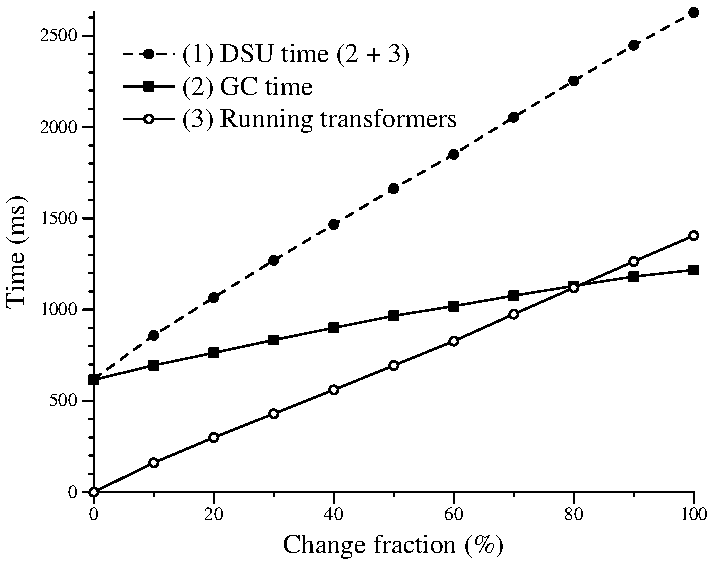
\includegraphics[scale=0.73]{100-graphs/microbench}
\hangcaption{Microbenchmark pause times with a heap size of 1280 MB containing
3.67 million objects\label{fig:microbench}}
\VspaceFixForHangcaption
\end{center}
\end{figure}


Table~\ref{tab:microbench} shows the elapsed time while varying the number
of total objects and the fraction of the objects that are updated.  The
variance was insignificant, so we do not report it.  The first group of
rows reports garbage collection time, the second group reports the time to
transform all updated objects, and the final group reports the total update
time. While the total time includes the time to load and install the
updated classes, synchronize running threads, and find a DSU safe point, it
is roughly equal to the sum of GC time and transformation time.  The first
column of the table shows the number of objects in the test, and the second
column the heap size, which is five times the minimum heap size to run the
microbenchmark. Columns 4 though 14 show pause times for varying fractions
(from 0\% to 100\%) of updated objects. 

To shed light on the results in the table, Figure~\ref{fig:microbench}
plots collection time, transformer time, and total update time for the
microbenchmark with 3.67 million objects in a 1280 MB heap.  The figure
shows that the costs of garbage collection and transformation increase  as
a function of the number of changed objects.  The slope of the ``GC time''
line illustrates the cost to deal with one object of the update type.  This
cost includes creating an additional copy of the transformed object;
creating an update log entry with a pointer to the old and new copy; and
caching a pointer to the old copy from the new copy. The slope of the
``Running transformers'' line illustrates the cost of accessing the update
log and actually running the transformer for one object.  This extra
processing to handle transforming objects increases the total pause time
with all objects updated by roughly four times compared to the pause time
with no object updated.  The ``Running Transformers'' line is steeper than
the ``GC time'' line, revealing that the cost of running transformers is
higher than the extra copying cost incurred during GC\@.

Transformations are more expensive than standard copying GC. The GC uses a
highly optimized {\tt memcopy} like code, whereas our transformer functions
use reflection to look up the \texttt{jvolveObject} function of the right
type, and this function copies one field at a time. One optimization would
be to eliminate the log by copying the old and new objects to their own
space and walking through and transforming each object.  The cost of
reflection could be reduced by caching the lookup, but even then a
na\"ively compiled field-by-field copy is much slower than the collector's
highly-optimized copying loop.  % Another possible optimization is to
% specially compile transformers to replace idiomatic use of copying
% assignments to contiguous fields by a \texttt{memcopy} over the
% corresponding range.


\section{Applications}

We now take a look at our three applications in detail. We present their
application structure, changes between versions, our success at updating
them, and some non-trivial transformer functions.

\subsection{Jetty webserver}
\label{subsec:jetty}

Jetty is a popular webserver written in Java. It supports static and
dynamic content and can be embedded within other Java applications. It is
used by various popular projects such as Eclipse, Google App Engine, and
the Hadoop map-reduce framework \cite{jetty-uses}.  \RVM, and thus \JV, is
not able to run the most recent versions of Jetty (6.x).  Therefore we
considered 11 versions, starting at 5.1.0, released in November, 2004
through 5.1.10, released in January, 2006.
% (the last % version prior to version 6).
Version 5.1.10 contains 317 classes and about 45,000 \SLOC (lines of code
excluding comments and blank lines, as reported by the sloccount
tool~\cite{sloccount, sloccount-wiki}).

\begin{table} \centering \footnotesize
\begin{tabular}{lrrccccrcc} \toprule
% First row
\mr{3}{5ex}{\BC Ver. \EC} &
\mr{3}{9ex}{\BC Date \EC} &
\mr{3}{7ex}{\BC SLOC \EC} &
\mr{3}{10ex}[2ex]{\BC \# classes added \EC} & \mc{6}{c}{\# changed} \\ \cmidrule{5-10}
% Second row 
       &                     &         &         & \mr{2}{*}{classes} & \mc{3}{c}{methods} & \mc{2}{c}{fields} \\ \cmidrule(lr){6-8} \cmidrule(lr){9-10}
       &                     &         &         &                    & add & del & \mc{1}{c}{chg}   & add & del \\ \midrule
5.1.0  & Nov 2004            & 42,981  &         &                    &     &     &                  &     &     \\
5.1.1  & Dec 2004            & 43,073  & 0       & 14                 &\ 4  & 1   &  38/0            &  0  & 0   \\
5.1.2  & Jan 2005            & 43,277  & 1       &\ 5                 &\ 0  & 0   &  12/1            &  0  & 0   \\
5.1.3* & Apr 2005            & 43,612  & 3       & 15                 & 19  & 2   &  59/0            & 10  & 1   \\
5.1.4  & Jun 2005            & 43,578  & 0       &\ 6                 &\ 0  & 4   &   9/6            &  0  & 2   \\
5.1.5  & Nov 2005            & 44,027  & 0       & 54                 & 21  & 4   & 112/8            &  5  & 0   \\
5.1.6  & Nov 2005            & 43,948  & 0       &\ 4                 &\ 0  & 0   &  20/0            &  5  & 6   \\
5.1.7  & Dec 2005            & 44,081  & 0       &\ 7                 &\ 8  & 0   &  11/2            &  9  & 3   \\
5.1.8  & Dec 2005            & 44,082  & 0       &\ 1                 &\ 0  & 0   &   1/0            &  0  & 0   \\
5.1.9  & Dec 2005            & 44,084  & 0       &\ 1                 &\ 0  & 0   &   1/0            &  0  & 0   \\
5.1.10 & Jan 2006            & 44,102  & 0       &\ 4                 &\ 0  & 0   &   4/0            &  0  & 0   \\ \bottomrule
\end{tabular}
\caption{Summary of updates to Jetty\label{tab:jetty-changes}}
\end{table}


Table~\ref{tab:jetty-changes} shows a summary of the changes in each
update. For each version, the first three columns list the version number,
release date and \SLOC. For versions 5.1.1 through 5.1.10,
each row tabulates the changes relative to the prior version. The fourth
column shows the number of classes that the new version added. The fifth
column shows the number of classes that contained changes from the previous
version. Columns 6 though 10 enumerate changes such as the addition,
deletion and modification of methods; and the addition and deletion of
fields. For the eighth column listing changed methods, the notation $x/y$
indicates that $x+y$ methods were changed, where $x$ changed in body only,
and $y$ changed their type signature as well. For dynamic updating systems
that only support changes to method bodies, only the first and last three
of the ten updates could be supported, since the rest either change method
signatures and/or add or delete fields.


\BCode[p]{0.72}
\begin{lstlisting}[frame=single]
// There are different listeners for various
// virtual hosts Each listener has multiple
// threads
public class HttpListener {
  public void run() {
    while (true) {
      if (job == null)
        wait();
      if (job != null)
        handle(job);
    }
  }
}

// Maps a collection of HttpListener objects
// which generates requests and HttpContext
// objects which maintain collection of
// HttpHandlers
public class HttpServer {
  public void start() {
    for (HttpContext c : contexts) {
      c.start();
    }
    for (HttpListener l : listeners) {
      l.start();
    }
  }

  public static void main(String args[]) {
    HttpServer server = new HttpServer();
    HttpContext context = server.getContext();
    context.addHandler(...);
    server.addListener(...);
    server.start();
  }
}
\end{lstlisting}
\ECode{Jetty webserver code: High level organization\label{fig:jetty-code}}


Figure~\ref{fig:jetty-code} shows the high-level organization of the
application. The main class of the application {\tt HttpServer} services
\HTTP requests by maintaining a map between a collection of \HttpListener
objects and {\tt HttpContext} objects. The \HttpListener
objects listen for client requests. The application supports virtual hosts
(multiple websites on the same server listening possibly at different
addresses) by having a \HttpListener object for each virtual host. The
listener also maintains a fixed pool of threads to service client requests,
thereby avoiding thread creation overhead for each request. The application
uses complex producer-consumer synchronization between the client sockets
and thread pools. {\tt HttpContext} objects provide context such as
filesystem path prefix, classpath, and resource location for {\tt
HttpHandler} objects. Each handler supports a different type of
request---regular file request, running servlets and web applications,
returning error messages, and so on. When the server is idle, threads in
the thread pools wait to be woken up by listeners which wait on client
sockets.


\subsubsection{State transformer functions in Jetty}

Between the default class and object transformers the \acf{UPT} generated
and those we wrote by hand, we successfully wrote dynamic updates to all
versions of Jetty that we examined. The update to version~5.1.2 demonstrates
the usefulness of automatically generated default transformers in the
common case. Version~5.1.2 changes the access protection of method {\tt
setHttpContext} in class {\tt HttpResponse} to \public. This method is now
called by methods outside class {\tt HttpResponse}
and \JV correctly loads these method bodies to
update the application. Since the update changes the class signature of
{\tt HttpResponse}, the entire class has to be reloaded again, and \JV must
run class and object transformers for this class.
Figure~\ref{fig:jetty-update-to-5.1.2} shows the default transformer that
\UPT generated.
In this situation, where
there is no semantic change, the default transformers
correctly set the fields in the new version. Moreover, the fact that the
{\tt HttpResponse} class has over fifty fields make the default
transformers extremely useful.

\begin{figure}[t]
\centering
\begin{minipage}{0.98\textwidth}
\begin{lstlisting}[frame=single]
import org.mortbay.http.HttpResponse;
import org.mortbay.http.r_5_1_1_HttpResponse;

public final class JvolveTransformers {
  public static void jvolveObject(HttpResponse to,
                          r_5_1_1_HttpResponse from) {
    to._status = from._status;
    to._reason = from._reason;
    to._httpContext = from._httpContext;
  }
  public static void jvolveClass(HttpResponse unused) {
    HttpResponse.log = r_5_1_1_HttpResponse.log;
    HttpResponse.__100_Continue =
          r_5_1_1_HttpResponse.__100_Continue;
    HttpResponse.__101_Switching_Protocols =
          r_5_1_1_HttpResponse.__101_Switching_Protocols;
    ...
    HttpResponse.__505_HTTP_Version_Not_Supported =
          r_5_1_1_HttpResponse.__505_HTTP_Version_Not_Supported;
    HttpResponse.__507_Insufficient_Storage =
          r_5_1_1_HttpResponse.__507_Insufficient_Storage;
    HttpResponse.__statusMsg =
          r_5_1_1_HttpResponse.__statusMsg;
    HttpResponse.__Continue =
          r_5_1_1_HttpResponse.__Continue;
  }
}
\end{lstlisting}
\end{minipage}
\hangcaption{UPT-generated transformers for the update to Jetty v5.1.2}
% These transformers were correct and used for the update.}
\label{fig:jetty-update-to-5.1.2}
\VspaceFixForHangcaption
\end{figure}


\lstset{frame=single}
\begin{figure}[p]
\begin{tabular}{@{}m{0.5\textwidth}@{}m{0.5\textwidth}@{}}
\BC \begin{minipage}{0.42\textwidth}
\begin{lstlisting}
public class HttpContext {
  private List
    _systemClasses;
}
\end{lstlisting}
\end{minipage} \EC &
\BC \begin{minipage}{0.42\textwidth}
\begin{lstlisting}
public class HttpContext {
  private String[]
    _systemClasses =
      new String [] {...};
}
\end{lstlisting}
\end{minipage} \EC \\[-3.5ex]
\BC (a) Version 5.1.5 \EC &
\BC (b) Version 5.1.6 \EC \\
\end{tabular}

\begin{tabular}{@{}b{\textwidth}@{}}
\centering
\begin{minipage}{0.7\textwidth}
\begin{lstlisting}
public static void jvolveObject(
  HttpContext to, r_5_1_5_HttpContext from) {
    to._systemClasses = null;
}
\end{lstlisting}
\end{minipage} \\[-0.5ex]
(c) Default transformer \\[1.5ex]
\begin{minipage}{0.7\textwidth}
\begin{lstlisting}
public static void jvolveObject(
  HttpContext to, r_5_1_5_HttpContext from) {
  if (from._systemClasses == null) {
    to._systemClasses = null;
  } else {
    to._systemClasses =
      new String[from._systemClasses.size()];
    int i = 0;
    for (Object o : from._systemClasses) {
      to._systemClasses[i] = (String) o;
      i++;
    }
  }
}
\end{lstlisting}
\end{minipage} \\[-0.5ex]
(d) User generated transformer
\end{tabular}
\caption{Object transformer from Jetty version 5.1.5 to
5.1.6\label{fig:sjt}}
\end{figure}
\lstset{frame=none}


We now describe updates where default transformers were not sufficient.  In
Version~5.1.3 class {\tt NCSARequestLog} added two boolean fields {\tt
\_logLatency} and {\tt \_logCookies}. {\tt \_logLatency} specifies whether
the application should include the latency to process HTTP requests when it
logs information about a request, and {\tt \_logCookies} controls whether
or not that application logs
cookies information. The default transformer sets these boolean
fields to {\tt false}. However, the actual values to set these fields to
depend on the configuration parameters when running the new version. In
the same update, Class {\tt Pool} which manages a pool of threads to handle
HTTP requests adjusts the number of threads based on system load, added a
\private field {\tt \_lastShrink} to store the time the number of threads
were last shrunk. Jetty uses this field to prevent shrinking
available threads frequently.  Setting this field to the default value of
zero should not pose any major problems because this field will have the
correct time the next time the pool is shrunk.

The update from version~5.1.5 to 5.1.6 changed the type of two fields {\tt
\_systemClasses} and {\tt \_serverClasses} from {\tt List} in the old
version to \StringArray in the new, in class {\tt HttpContext}.
Figure~\ref{fig:sjt} shows the changes to one of these fields. In
Figure~\ref{fig:sjt}~(c), \UPT's default transformer sets the field {\tt
\_systemClasses} to \NULL (similar to the example with JavaEmailServer,
Figure~\ref{fig:jes-transformer-code}). Since the new version's field
declaration (Figure~\ref{fig:sjt}~(b)) already declares the value of these
fields, the developer writing to object transformer has to decide whether
to use this value or convert the value stored in the old version's list
into a String array. We choose the latter option, shown in
Figure~\ref{fig:sjt}~(d).

\subsubsection{Reaching a safe point in Jetty}

\begin{sidewaystable} \centering \footnotesize
\begin{tabular}{@{}lcrrrrrrr@{}} \toprule
\CC{Upd.}   &                & \CC{Number of}  & \mc{4}{c}{\# methods not allowed on stack, due to}        & \mc{2}{c}{Number of}   \\ \cmidrule{4-7}
\CC{to}     & Reached        & \CC{methods at} & \CC{class}   & \CC{method}  & \CC{indirect} &             & \mc{2}{c}{restricted}  \\
\CC{ver.}   & safe point?    & \CC{runtime}    & \CC{updates} & \CC{body}    & \CC{method}   & \CC{Total}  & \mc{2}{c}{methods}     \\ \cmidrule{8-9}
            &                &                 &              & \CC{updates} & \CC{updates}  &             & \mc{1}{c}{w/o OSR}
                                                                                                                      & \mc{1}{c}{w/ OSR}\\ \toprule
5.1.1   &  always        & 1378 (376) & 26/49          & 7/12           & 20/29           & 53/90  (17)  & 67         & 10         \\
5.1.2   &  4/5$^\dagger$ & 1374 (375) & 25/25          & 3/5            & 35/43           & 63/73  (35)  & 67         & 4          \\
5.1.3   &  0/5$^*$       & 1374 (375) & 326/382        & 4/6            & 42/45           & 370/433 (97) & 373        & 23         \\
5.1.4   &  always        & 1384 (374) & 82/82          & 5/6            & 15/16           & 101/104 (24) & 101        & 10         \\
5.1.5   &  always        & 1380 (372) & 14/80          & 39/60          & 13/15           & 62/155 (17)  & 62         & 60         \\
5.1.6   &  3/5$^\dagger$ & 1394 (378) & 203/219        & 3/3            & 16/19           & 222/241 (40) & 223        & 20         \\
5.1.7   &  always        & 1394 (380) & 186/187        & 1/2            & 53/69           & 239/258 (74) & 243        & 12         \\
5.1.8   &  always        & 1402 (379) & 0/0            & 1/1            & 0/0             & 1/1   (1)    & 1          & 1          \\
5.1.9   &  always        & 1402 (379) & 0/0            & 0/1            & 0/0             & 0/1   (0)    & 0          & 0          \\
5.1.10  &  always        & 1402 (379) & 0/0            & 4/5            & 0/0             & 4/5   (2)    & 6          & 4          \\ \bottomrule
\mc{9}{c}{\begin{minipage}{0.6\textwidth}
\vspace{2ex}
$^\dagger$Restricted method \texttt{HttpConnection.handleNext()} was active
\end{minipage}} \\[1ex]
\mc{9}{c}{\begin{minipage}{0.6\textwidth}
$^*$Restricted method \texttt{ThreadedServer.acceptSocket()} was always active
\end{minipage}} \\
\end{tabular}
\caption{Impact of safe point restrictions on updates to Jetty}
\label{tab:safe-point-jetty}
\end{sidewaystable}

% vim:tw=0


For the updates we considered, we tried to study how our safe point
restrictions (Section~\ref{sec:safe}) inhibited a dynamic update.
Other than the update to 5.1.3, all versions immediately
reached a safe point every time, with no need of return barriers.

% To understand why, we instrumented the VM to emit information about
% restricted method set and, if a safe point cannot be reached, which
% restricted method was active. 

% \suriya{The following information about inlining is commented out. What
% should we do with this? See .tex file}

For each version, starting at 5.1.0, we ran Jetty under 20\% load (160
connections per second from our httperf experiments). After 30 seconds we
tried to apply the update to the next version; if a safe point could not be
immediately reached, we deemed the attempt as failed. We tried five such
attempts for each version, starting up from the server from scratch for
each attempt. The results are presented in
Table~\ref{tab:safe-point-jetty}. Column 2 shows the number of times out of
five such runs where the application reached a safe point. The methods
whose presence on a thread stack precluded the application from reaching a
safe point are mentioned below the table. For the update to 5.1.3, the
offending method was always active because it contained an infinite loop.
The other updates either always succeeded, or did after a small number of
retries.

We could not apply the update to version 5.1.3 (denoted with an asterisk in
the table) because \JV was never able to reach a safe point. The update
modified {\tt ThreadedServer.acceptSocket()}, a method that waits for a
connection from the client, and this method is nearly always on stack.  We
installed a return barrier that is triggered when {\tt acceptSocket}
returns, but this barrier is not sufficient to perform the update since the
main methods of several threads were themselves modified. For example, we
also install a return barrier on {\tt PoolThread.run()}, but this barrier
is never triggered because this method never becomes inactive.

Column 3 contains the total number of methods in the program at runtime,
where the number in parentheses is the number of those which the compiler
inlined when using aggressive optimization.  This provides an upper bound
on the effect of inlining in reaching a safe point.  The next group of
columns contains the restricted method set. Each column in the group
specifies the number of methods loaded at run time by the \VM, followed by
the total number of methods in that category in the program. The first
column in this group is the number of methods in classes involved in a
class update. Recall that when a class is updated, say by adding a field,
all its methods are considered restricted (see section~\ref{sec:safe}).  The
second column in this group is the number of methods whose bodies are
updated, the third is the number of category~(2) or indirectly updated
methods, and the
fourth sums these, with the number of methods that were inlined written in
parentheses. The final two columns list the total number of methods in the
restricted set; they differ from the first number in the fourth column by
the number of inlined callers of the restricted methods that were not
already restricted.  The final column lists the actual number of restricted
methods when \JV's \OSR capability is enabled.

The table shows that both indirect method calls and inlining significantly
add to the size of the restricted set.  Inlining though, is small by
comparison, because all callers of an updated class's methods are
\emph{already} included in the indirect set. Therefore, inlining these
methods adds no further restriction.  In most cases \OSR support
dramatically reduces the number of restricted methods and increases the
likelihood of reaching a \USD safe point.  Interestingly, having a greater
number of restricted methods overall does not necessarily reduce the
likelihood that an update will take effect; rather, it depends on the
frequency with which methods in this set are on the stack.

% REFACTOR: add para back if we get things to work.
% We refactored the various long-running main methods in versions 5.1.2 and
% 5.1.3 to extract the modified bodies of long running methods into separate
% methods and leave the main method containing the loop unmodified between
% the two versions.  (This sort of transformation is performed by other
% systems automatically by programmer directive in
% Ginseng~\cite{neamtiu06dsu}.) 
% When we attempted to perform a dynamic update, \DSU{}
% installed a return barrier for {\tt acceptSocket()}. This function waits
% for a connection and returns after a timeout. \DSU{} was able to update the
% application when this function returned. 

\begin{table}[t] \footnotesize \centering
\begin{tabular}{lrrcccccrcc} \toprule
% First row
\mr{3}{5ex}{\BC Ver. \EC} &
\mr{3}{9ex}{\BC Date \EC} &
\mr{3}{7ex}{\BC SLOC \EC} & \mc{2}{c}{\# classes} & \mc{6}{c}{\# changed} \\ \cmidrule{4-5} \cmidrule(l){6-11}
% Second row 
       &                     &         & \mr{2}{*}{add} & \mr{2}{*}{del}      & \mr{2}{*}{classes} & \mc{3}{c}{methods} & \mc{2}{c}{fields} \\ \cmidrule(lr){7-9} \cmidrule(lr){10-11}
       &                     &         &       &       &                    & add & del & \mc{1}{c}{chg}   & add & del \\ \midrule
% \begin{tabular}{|l|r|r||c|c||c|r|c|r|r|c|} \hline \T
%       &                      &        & \mc{2}{c||}{\# classes} &    \mc{6}{c|}{\# changed} \\
% Ver.  & \mc{1}{c|}{Date}     & SLOC   & add & del & classes & \mc{3}{c|}{methods} & \mc{2}{c|}{fields} \\
%       &                      &        &     &     &         & add & del & chg   & add & del \\ \hline \hline \T
1.2.1 & Dec 2002             &  2,841 &     &     &         &     &     &       &     &     \\
1.2.2 & Feb 2003             &  2,841 & 0   & 0   & 3       & 0   & 0   & 3/0   & 0   & 0   \\
1.2.3 & Jul 2003             &  2,924 & 0   & 0   & 7       & 0   & 0   & 14/2  & 12  & 0   \\
1.2.4 & Sep 2003             &  2,961 & 0   & 0   & 2       & 0   & 0   & 4/0   & 0   & 0   \\
1.3*  & Oct 2003             &  2,305 & 4   & 9   & 2       & 11  & 3   & 6/9   & 12  & 5   \\
1.3.1 & Oct 2003             &  2,307 & 0   & 0   & 2       & 0   & 0   & 4/0   & 0   & 0   \\
1.3.2 & Nov 2003             &  2,359 & 0   & 0   & 8       & 4   & 2   & 4/2   & 3   & 1   \\
1.3.3 & Nov 2003             &  2,368 & 0   & 0   & 4       & 0   & 0   & 3/0   & 0   & 0   \\
1.3.4 & Feb 2004             &  2,447 & 0   & 0   & 6       & 2   & 0   & 6/0   & 2   & 0   \\
1.4   & Jul 2004             &  2,529 & 0   & 0   & 7       & 6   & 1   & 4/1   & 6   & 0   \\ \bottomrule
\end{tabular}
\caption{Summary of updates to JavaEmailServer\label{tab:jes-changes}}
\end{table}


\subsection{JavaEmailServer}
\label{subsec:jes}

For JavaEmailServer, we considered 10 versions---1.2.1 through
1.4---spanning a duration of about two years.  Version 1.4 consists of 20
classes and about 2500 \SLOC.  Table~\ref{tab:jes-changes} shows the
release date, source lines of code and summary of updates to each new
version.

Figure~\ref{fig:jes-code} shows the
high-level structure of JavaEmailServer's code. The application creates
multiple \POP and \SMTP protocol handler threads. The number of threads can
be configured by the user. Each thread listens on its respective port (110
for \POP and 25 for \SMTP), waiting for new client connections. Upon
receiving a client request, the server thread communicates with the client,
services the client's command, and goes back to listening again. The
main loop of \POP and \SMTP servers are in {\tt Pop3Processor.run()} and
{\tt SMTPProcessor.run()} respectively. The \POP server authenticates
users, reads their e-mail messages from the filesystem and sends them to
the client through the network. The \SMTP server reads in e-mail messages
from the network and writes them to the filesystem. These messages may be meant
to be delivered to local users or relayed to other servers on the internet.
Message delivery is handled by a single {\tt SMTPSender} thread, which
polls the filesystem for new messages and writes them into user mailboxes,
or relays them to other servers. The number of threads and therefore the
maximum number of clients that can simultaneously be serviced is fixed and
known when the application starts. The server will ignore clients that try
to connect when all server threads are responding to requests. At any
moment, the {\tt run()} methods of all threads and based on server load,
additional methods to handle the \POP and \SMTP protocols and methods to
deliver messages are active on stack.

\BCode[p]{0.75}
\begin{lstlisting}[frame=single]
// Listen on socket for POP client connections
// Handle a client
public class Pop3Processor implements Runnable {
  public void run() {
    while (true) {
      Socket client = serverSocket.accept();
      handleCommands();
    }
  }
}

// SMTPProcessor is similar to Pop3Processor

// Poll the filesystem and deliver messages
public class SMTPSender implements Runnable {
  public void run() {
    while (true) {
      if (messageToBeDelivered)
        deliverMessages();
      sleep();
    }
  }
}

public class Mail {
  public static void main(String args[]) {
    // Create 5 POP threads
    for (int i = 0; i < 5; i++)
      new Thread(new Pop3Processor()).start();

    // Create 5 SMTP threads
    for (int i = 0; i < 5; i++)
      new Thread(new SMTPProcessor()).start();

    // Create one thread that delivers mail
    new Thread(new SMTPSender()).start();
  }
}
\end{lstlisting}
\ECode{JavaEmailServer code: High level organization\label{fig:jes-code}}


\subsubsection{Updates to JavaEmailServer}
Approaches that only support updates to method bodies will be able to
handle only four of the updates shown in Table~\ref{tab:jes-changes}.  We
could successfully construct updates for all versions we examined and we
could successfully apply all of them except the update to version 1.3. For
all updates but the one from 1.3.1 to 1.3.2 (shown in
Figure~\ref{fig:jes-string-emailaddress-example}), default transformers were
sufficient.


Version 1.3 has 20\% fewer \SLOC than its prior version because the update
reworked the entire
configuration framework of the server. Among other things, this version
removes a GUI tool for user administration and adds several new classes
that implement a file-based configuration system. As a result, many
classes are modified to point to a new configuration object.  Among these
classes are threads with infinite processing loops that accept POP and SMTP
requests.  Because these threads are always active, the safety condition
can never be met and thus the update cannot be applied.

The update from 1.3.1 to 1.3.2 indirectly changes the
\SMTPSenderrun
and \texttt{Pop3Processor.run()} methods.  These
methods contain processing loops run by several threads.  Though these
methods are always running, \JV applies \OSR and the update succeeds.  \JV
also uses OSR for the update from 1.3.2 to 1.3.3.
%MWH: suriya says this statement just isn't true.  Updates fine.  A method
%used to process connections was also changed, and this method is
%frequently active when the server is under load.  (A similar method was
%changed in the update to version 1.3.3.)  A return barrier installed on
%this method permits the update to take effect.  

\BCode[p]{0.75}
\begin{lstlisting}[frame=single]
public class FtpServer implements Runnable {
  // main loop of server
  public void run() {
    while (true) {
      Socket cl = serverSocket.accept();
      RequestHandler rh = new RequestHandler(cl);
      (new Thread(rh)).start();
    }
  }
}

// Handle a single client
public class RequestHandler implements Runnable {
  private BufferedReader reader;
  private FtpWriter writer;
  private boolean isClosed;

  // main loop of server-client conversation
  public void run() {
    while (!isClosed) {
      String command = reader.readLine();
      service(command, writer);
    }
  }
}

// Creates a single server thread
public class CommandLine {
  public static void main(String args[]) {
    FtpServer server = new FtpServer();
    (new Thread(server)).start();
  }
}
\end{lstlisting}
\ECode{CrossFTP code: High level organization\label{fig:crossftp-code}}


\subsection{CrossFTP server}
\label{subsec:crossftp}

CrossFTP server is an easily configurable, security-enabled \FTP server.
CrossFTP allows simple configuration through a \GUI and more advanced
customization using configuration files. The \GUI interface also allows
detailed monitoring of server operation and a real-time look at active
clients and the commands they issue.  We did not use the GUI interface and
therefore do not consider changes to that part of the program.

\begin{table}[t] \footnotesize \centering
\begin{tabular}{lcccccccrcc} \toprule
     &  \mc{2}{c}{SLOC} & \mc{2}{c}{\# classes} &    \mc{6}{c}{\# changed}             \\ \cmidrule(l){2-3} \cmidrule(lr){4-5} \cmidrule{6-11}
Ver. & \mr{2}{*}{Total}   & \mr{2}{10ex}{Without JmDNS} & \mr{2}{*}{add} & \mr{2}{*}{del} & \mr{2}{*}{classes} & \mc{3}{c}{methods} & \mc{2}{c}{fields}  \\ \cmidrule{7-9} \cmidrule(l){10-11}
     &                    & &     &     &         & add & del & chg   & add & del             \\ \toprule
1.05 &  13,852            & 13,852   &     &     &         &     &     &       &     &                 \\
1.06 &  13,926            & 13,926   & 4   & 1   & 1       & 0   & 0   & 3/0   & 1   & 0               \\
1.07 &  18,081            & 14,066   & 0   & 0   & 3       & 4   & 0   & 14/0  & 5   & 0               \\
1.08 &  18,108            & 14,093   & 0   & 1   & 3       & 2   & 0   & 10/0  & 0   & 2               \\ \bottomrule
\end{tabular}
\caption{Summary of updates to CrossFTP server\label{tab:crossftp-changes}}
\end{table}

% vim:tw=0


We looked at 4 versions of CrossFTP---1.05 through 1.08, details shown in
Table~\ref{tab:crossftp-changes}---spanning a duration of more than a year.
Version 1.08 contains about 18,000 \SLOC across 161 classes.  Version 1.07
added over four thousand \SLOC by including code from JmDNS, a Java
implementation of multi-cast DNS~\cite{jmdns}. We did not exercise this
functionality in our runs. 

Figure~\ref{fig:crossftp-code} shows the high level organization of the
server's code. The server has one active thread, an instance of {\tt
FtpServer} which listens on a socket for client connections. The main loop
of the server is shown in function {\tt FtpServer.run()}. For each client,
the server spawns a new thread, an instance of the class {\tt
RequestHandler}.  At any point of time, the application is running one
server thread and multiple connection threads, one for each active client
connection. The main loop to handle a client is given in {\tt
RequestHandler.run()}. The server reads a command from the client, services
the command and waits for the next one. In steady state, {\tt FtpServer}'s
{\tt run} method, {\tt RequestHandler}'s {\tt run} method and methods
involved in processing particular \FTP commands from the client are active
on stack.

\subsubsection{Updates to CrossFTP}

\JV successfully applies all three updates to this application. For all
three updates, the default transformers we sufficient. Note that since all
updates either add or delete fields, simple method body updating support on
its own would be insufficient.

\JV could only apply the update from version 1.07 to 1.08 when the server
was relatively idle. The server runs a new {\tt RequestHandler} thread to
process each \FTP session, and the \texttt{RequestHandler.run()} method was
changed by the update. \JV installs a return barrier on this method, but
with many active sessions, this method is essentially always on stack,
preventing the update.


\section{Conclusion}

Our evaluation shows that
% \JV is one of the most efficient among dynamic updating systems.
\JV is the first full-featured dynamic updating system that imposes no
steady-state overhead. To perform an update, \JV pauses the application
for a modest time period, roughly equal to a full heap garbage collection
pause. \JV is the most versatile dynamic updating system for Java and
supports 20 of 22 real-world updates written over a one to two year period
to three open-source server programs.
